\documentclass{article}
\usepackage{graphicx, float}
\author{Astrid Augusta Yu}
\title{CPE 233 Lab \#1}
\date{2020 April 13}

\begin{document}
\maketitle

\section{Questions}
\begin{enumerate}
    \item One aspect of the modern digital design paradigm is 
    \item{
        Generally, the circuit can be described by its writer and its reader components. The writer is mostly active during the 
        calculate state (state 1 in the diagram) and the reader is mostly active during the display state (state 0 in the diagram).

        When the button is pressed, that is the \texttt{calculate} signal that tells the circuit to enter the calculate state.
        A specialized accumulator for Fibonacci numbers is reset, and on every clock cycle, it advances one step in the 
        Fibonacci sequence. 

        There is also an accumulator to keep track of what address to write the memory to. It is also reset when the 
        \texttt{calculate} signal is asserted. Every clock cycle, it steps one address forward.

        The Fibonacci accumulator and the write address accumulator are directly wired to the \texttt{data} and 
        \texttt{addr\_write} ports of the RAM respectively. However, nothing will get written if \texttt{en\_write} is not set
        by the FSM to 1, signaling write mode. During the calculate state, write is always enabled, but during display, it is disabled.
        
        The FSM receives the signal to stop calculating when its \texttt{fin} port is asserted. This happens when the 
        write address accumulator reaches 15. Once this happens, the FibWriter raises the \texttt{ready} status port,
        which enables the \texttt{univ\_sseg}.

        In the display state, there is another accumulator that is always incremented by 1 that controls the \texttt{addr\_read}
        port of the RAM. The RAM's read output is fed directly into the \texttt{cnt1} port of the univ\_sseg.

        I'll admit that there is a part of the design that is slightly awkward: the FSM would probably be better if it was in FibCalculator
        instead of FibWriter. This way there is better separation of concerns and the design would be more modular.
    }
    \item{ 
        There are 17 clock cycles required, calculated as follows:

        \begin{tabular}{| p{8cm} | r |}
            \hline
            \textbf{Event(s)} & \textbf{Clock Cycles} \\
            \hline
            Button press detected. Transition into calculate state. Set address to 0 and calculate its values. & 1 \\
            \hline
            Step up to address 15 inclusive and calculate numbers along the way. & 15 \\ 
            \hline
            \texttt{fin} is triggered. Transition into display state. & 1 \\
            \hline
            \textbf{TOTAL} & \textbf{17} \\
            \hline
        \end{tabular}
    }
    \item It would have to take another clock cycle after the state transition for the external device to react to the state transition.
    \item {
        I used a Moore-type FSM because all of its outputs are determined solely from the state. Moore-type FSMs are generally more predictable
        than Mealy-type FSMs because of this property, which is why I ended up doing it this way. 
        
        I was originally going to make a Mealy-type FSM, but I found out
        while I was debugging my design that I could replace the Mealy FSM with an equivalent Moore FSM without losing clock cycles.
    }
    \item {
        By implementing an FSM that has less states, it becomes easier to reason about the state transitions. For a Moore-type machine with $n$,
        states, there could be a maximum of $2^n$ state transitions. It get worse for Mealy-type machines because not all transitions to a certain
        state will produce the same set of ouptuts. By using less states, there is less effort involved in verifying that the machine works correctly.
    }
    \item {
        Propagation delay is probably what would limit the maximum theoretical circuit speed. It takes time for electrons to pass from one gate to
        another, so we can't indefinitely decrease the period of our clock, otherwise we will have faulty, unsaturated signals.
    }

\end{enumerate}

\section{Programming Assignment}

\begin{verbatim}
#include <stdio.h>

int main() {

    // Declare memory
    int mem[16];
   
    // Accumulator variables
    int prev = 0;
    int sum = 1;

    // Generate fibonacci and write to memory
    for (int i = 0; i < 16; i++) {
        mem[i] = sum;
        int tmp = prev;
        prev = sum;
        sum += tmp;
    }

    // Read from memory sequentially, displaying address
    for (int i = 0; i < 16; i++) {
        printf("%d\t%d\n", i, mem[i]);
    }

    return 0;
}
\end{verbatim}

\section{Hardware Design Assignment}

We are summing $16$ 8-bit integers. Therefore we need $n=12$ bits to store them.

Proof:

$2^n = 16 \dot (2^8 - 1)$

$n = log_2(16 \dot (2^8 - 1)) \approx 12$

\begin{figure}[H]
    \centering
    \textbf{FSM}
    \includegraphics[width=\linewidth]{fsm-2.jpg}
\end{figure}

\begin{figure}[H]
    \centering
    \textbf{Block Diagram}
    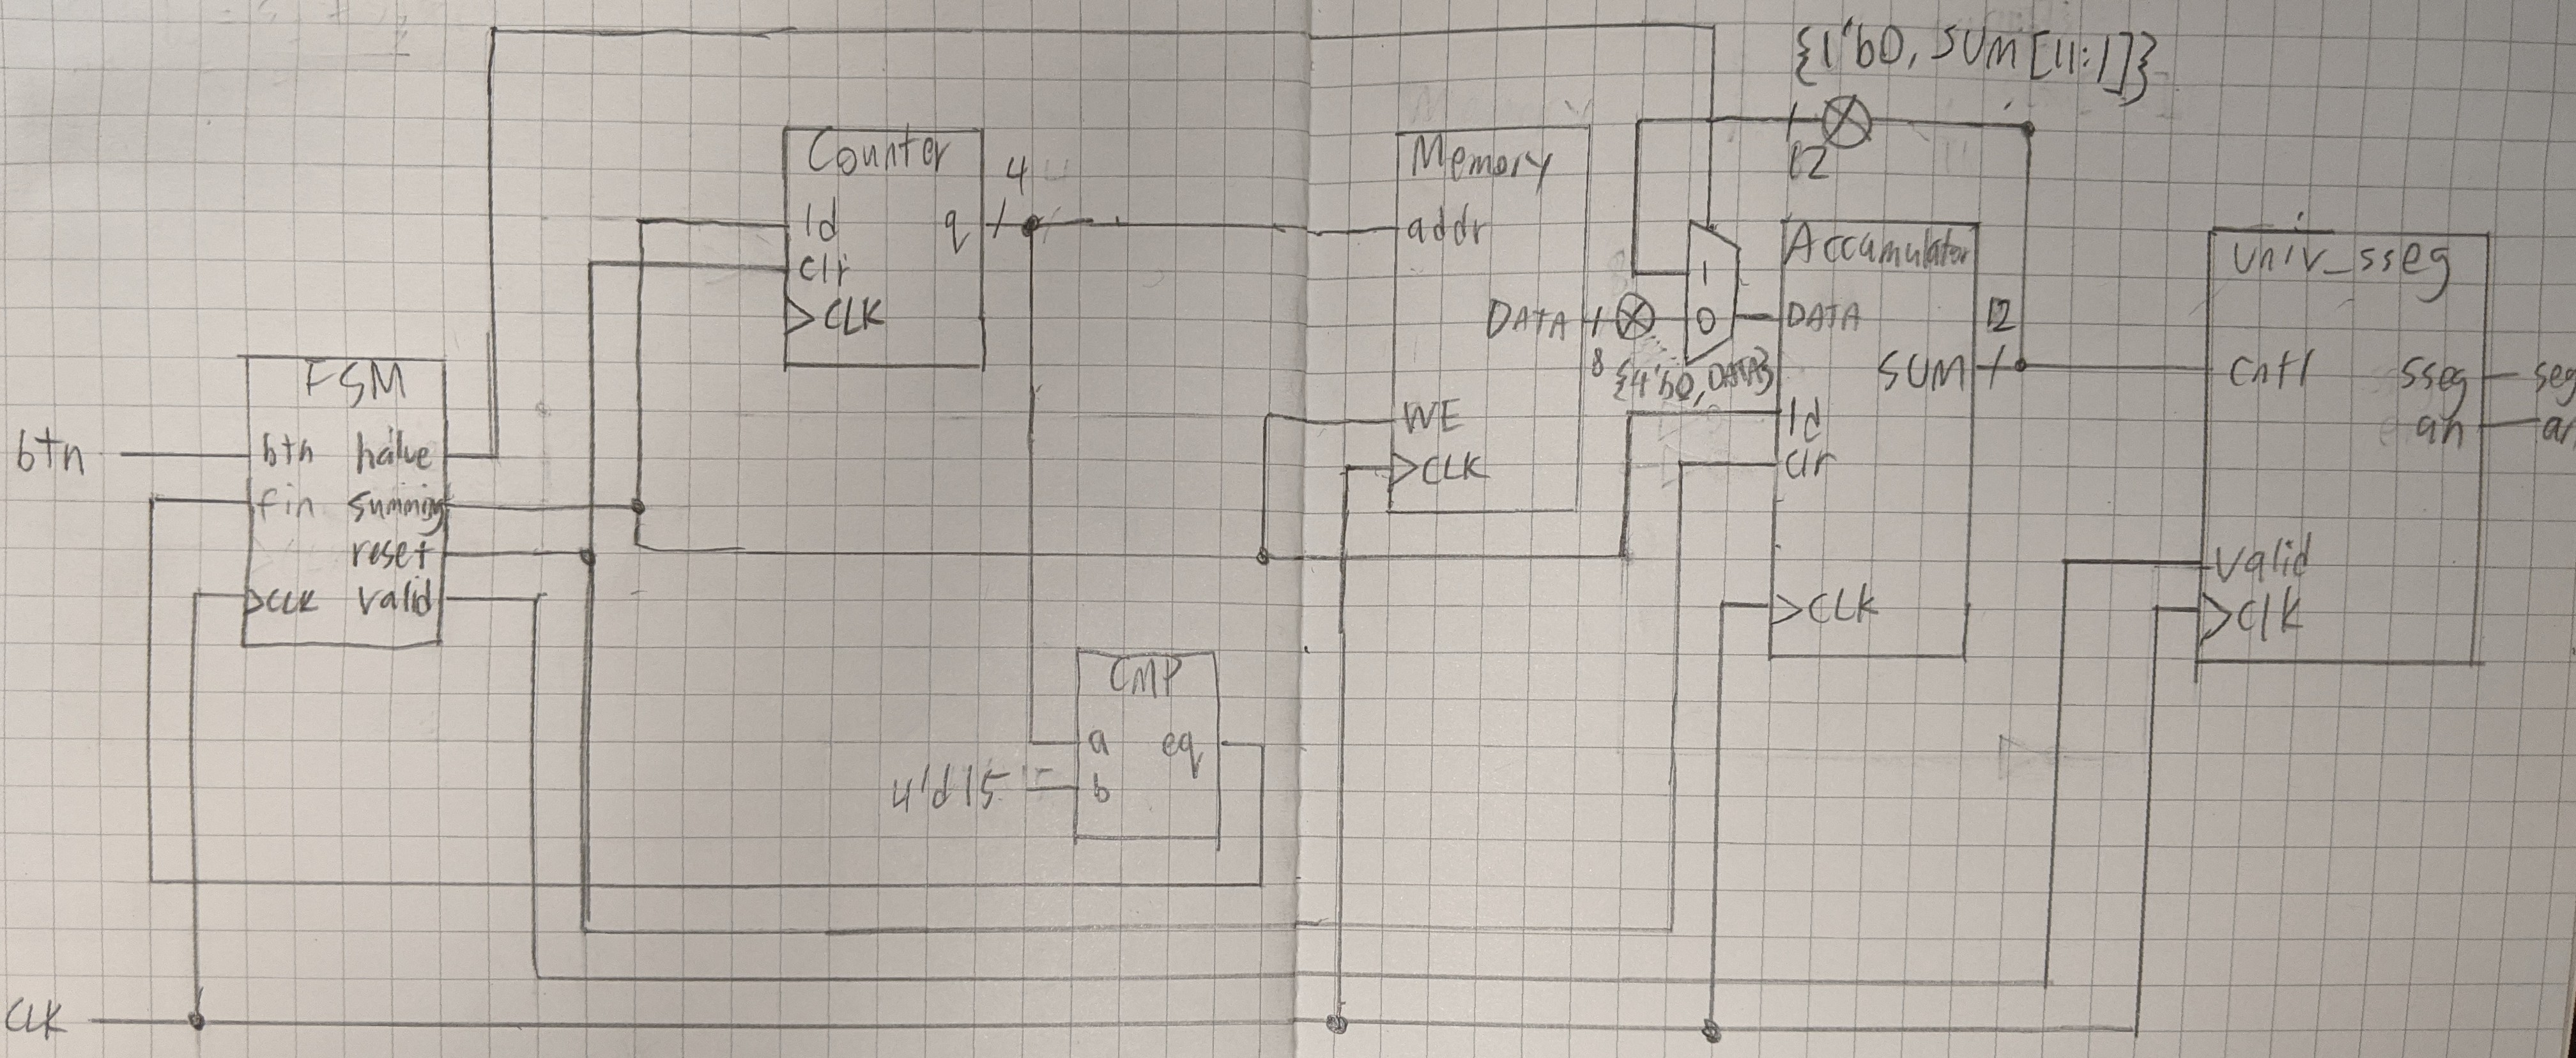
\includegraphics[width=\linewidth]{bd-2.jpg}
\end{figure}

\section{Black Box Diagrams}

\begin{figure}[H]
    \centering
    \textbf{Top.sv}
    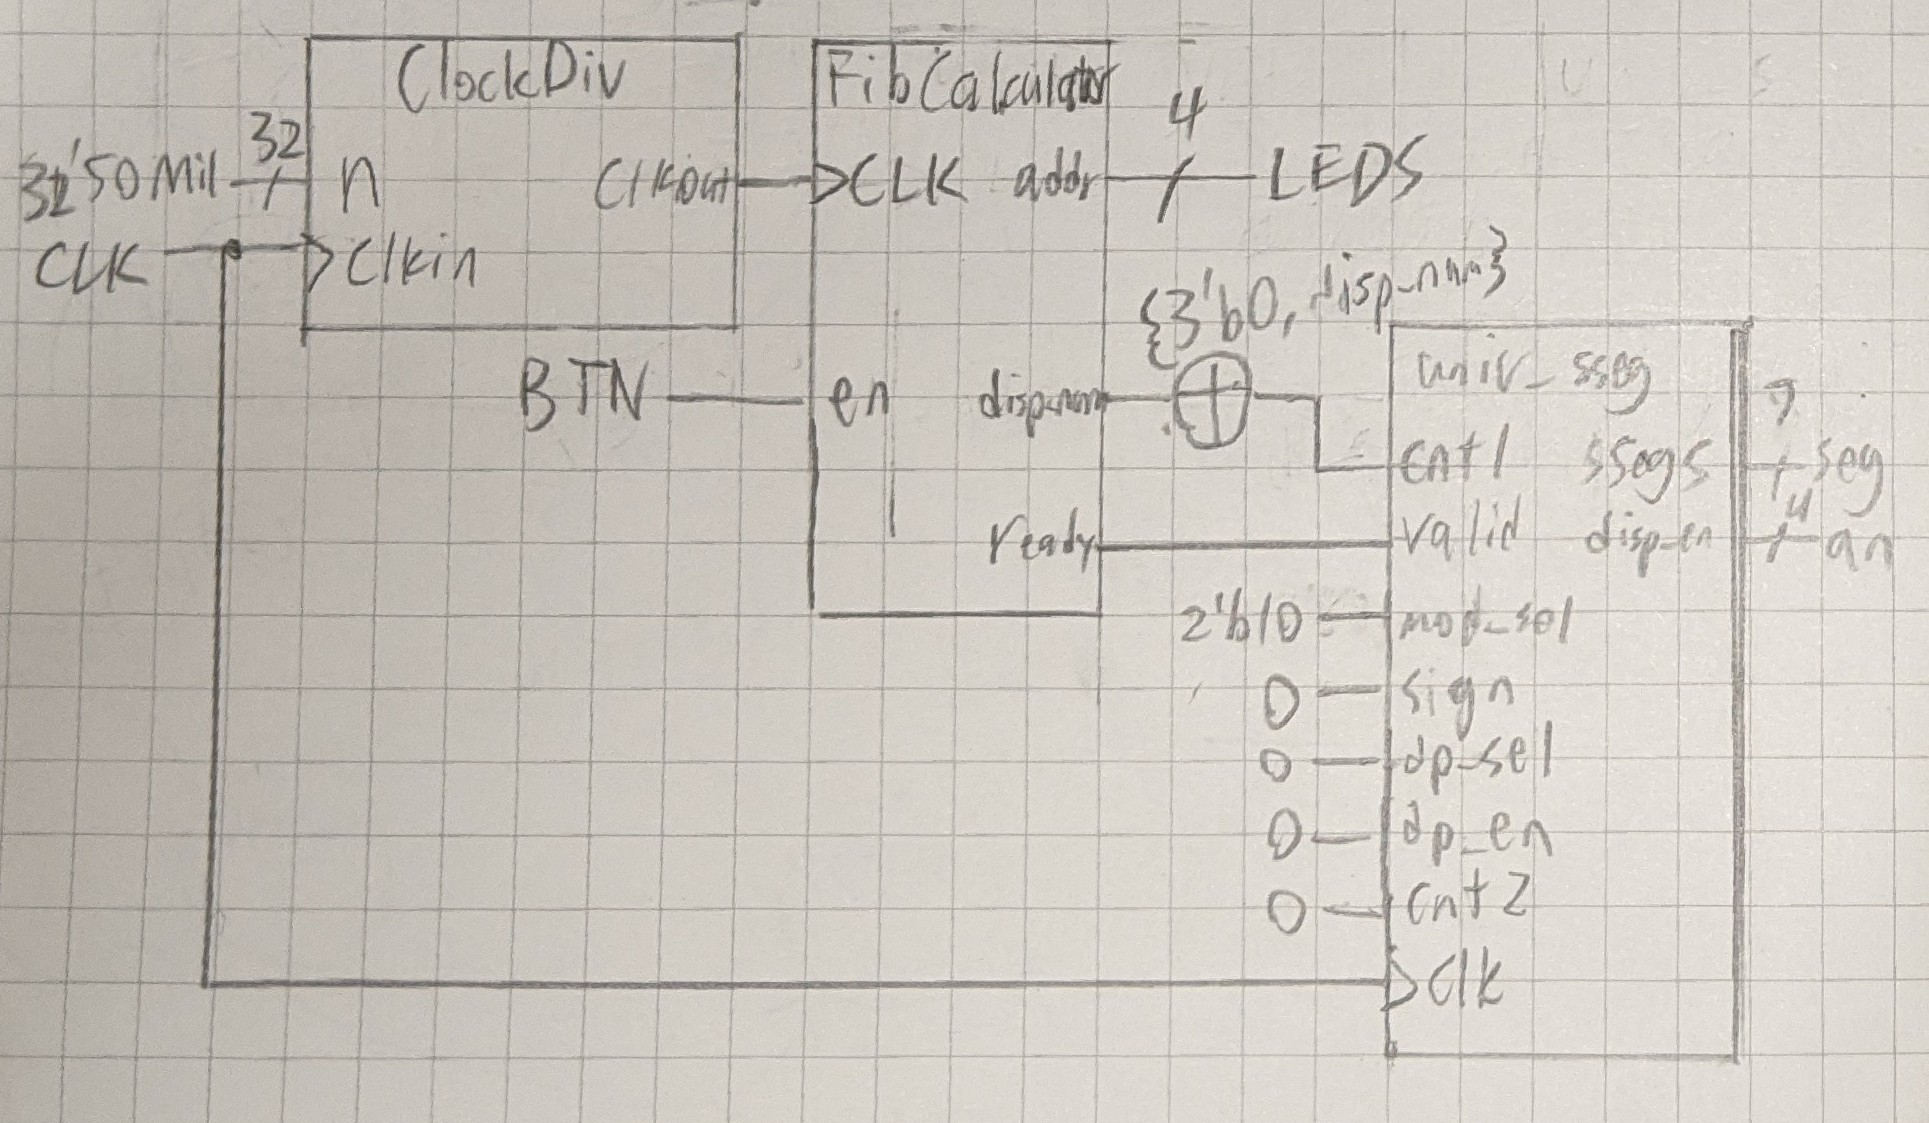
\includegraphics[width=\linewidth]{top.jpg}
\end{figure}

\begin{figure}[H]
    \centering
    \textbf{FibCalculator.sv}
    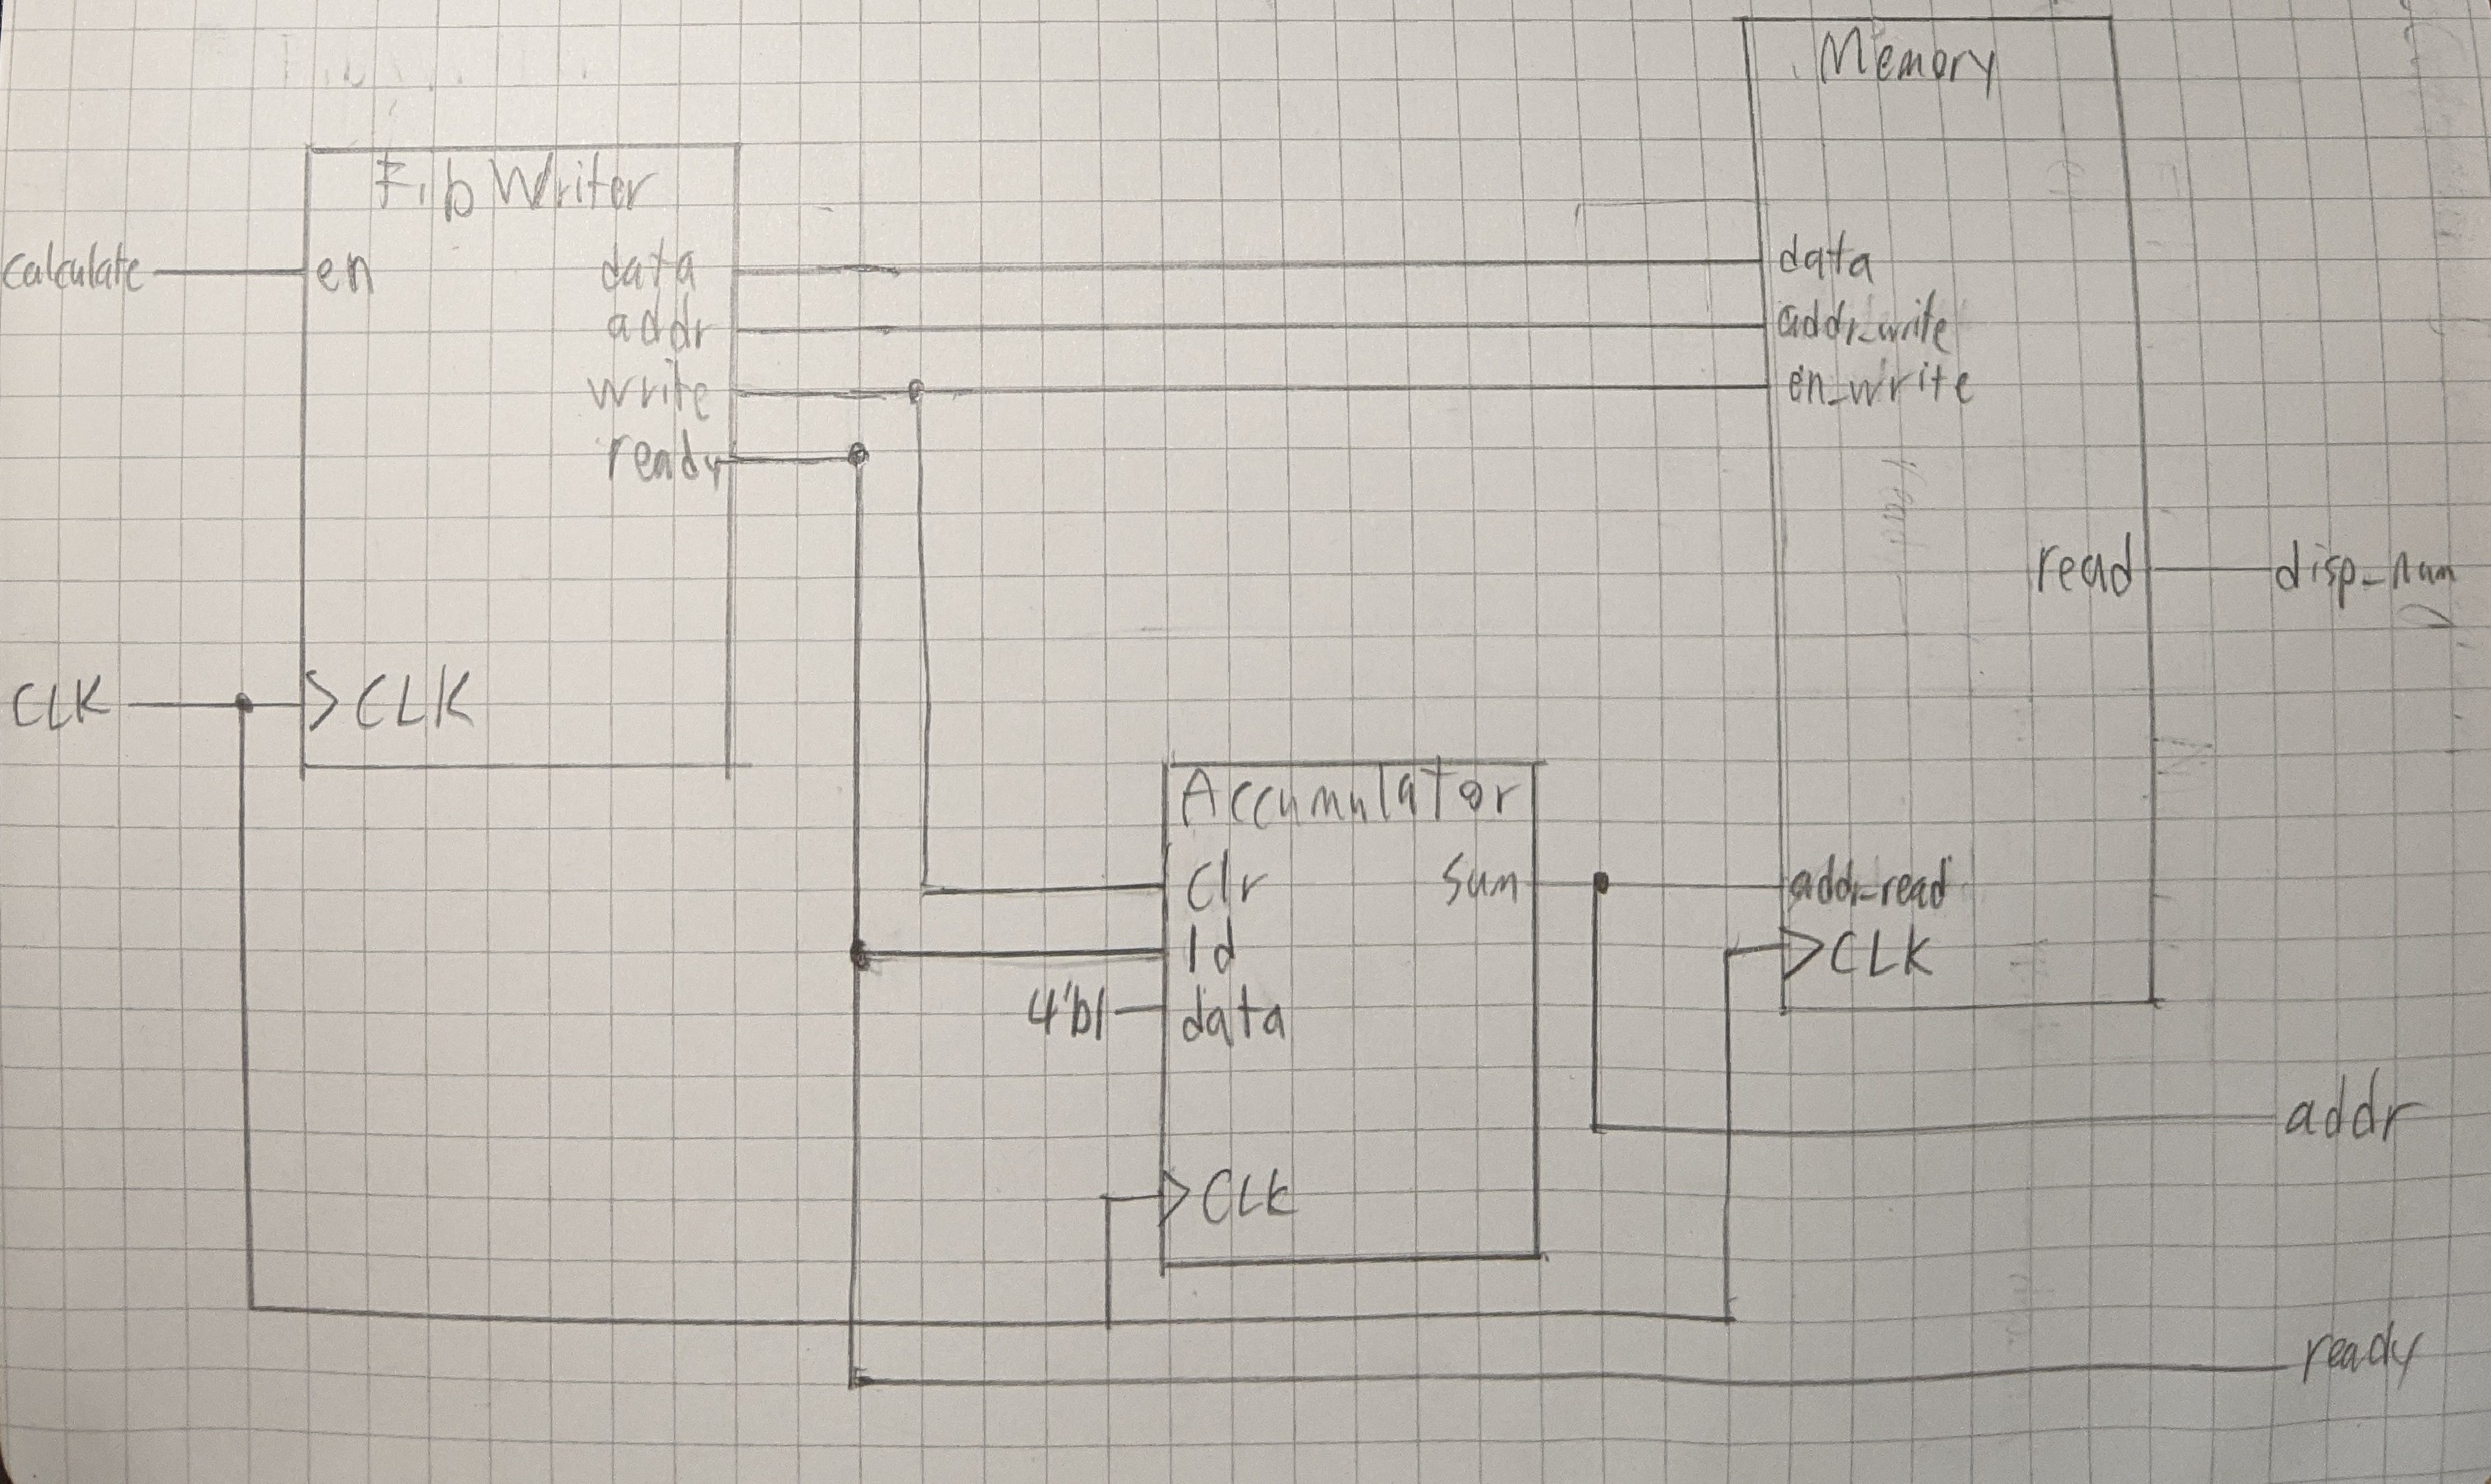
\includegraphics[width=\linewidth]{fibcalc.jpg}
\end{figure}

\section{HDL Code}

The SystemVerilog code used to generate this circuit can be found in the 
attached .zip file.

\section{State Diagram}
\begin{figure}[H]
    \centering
    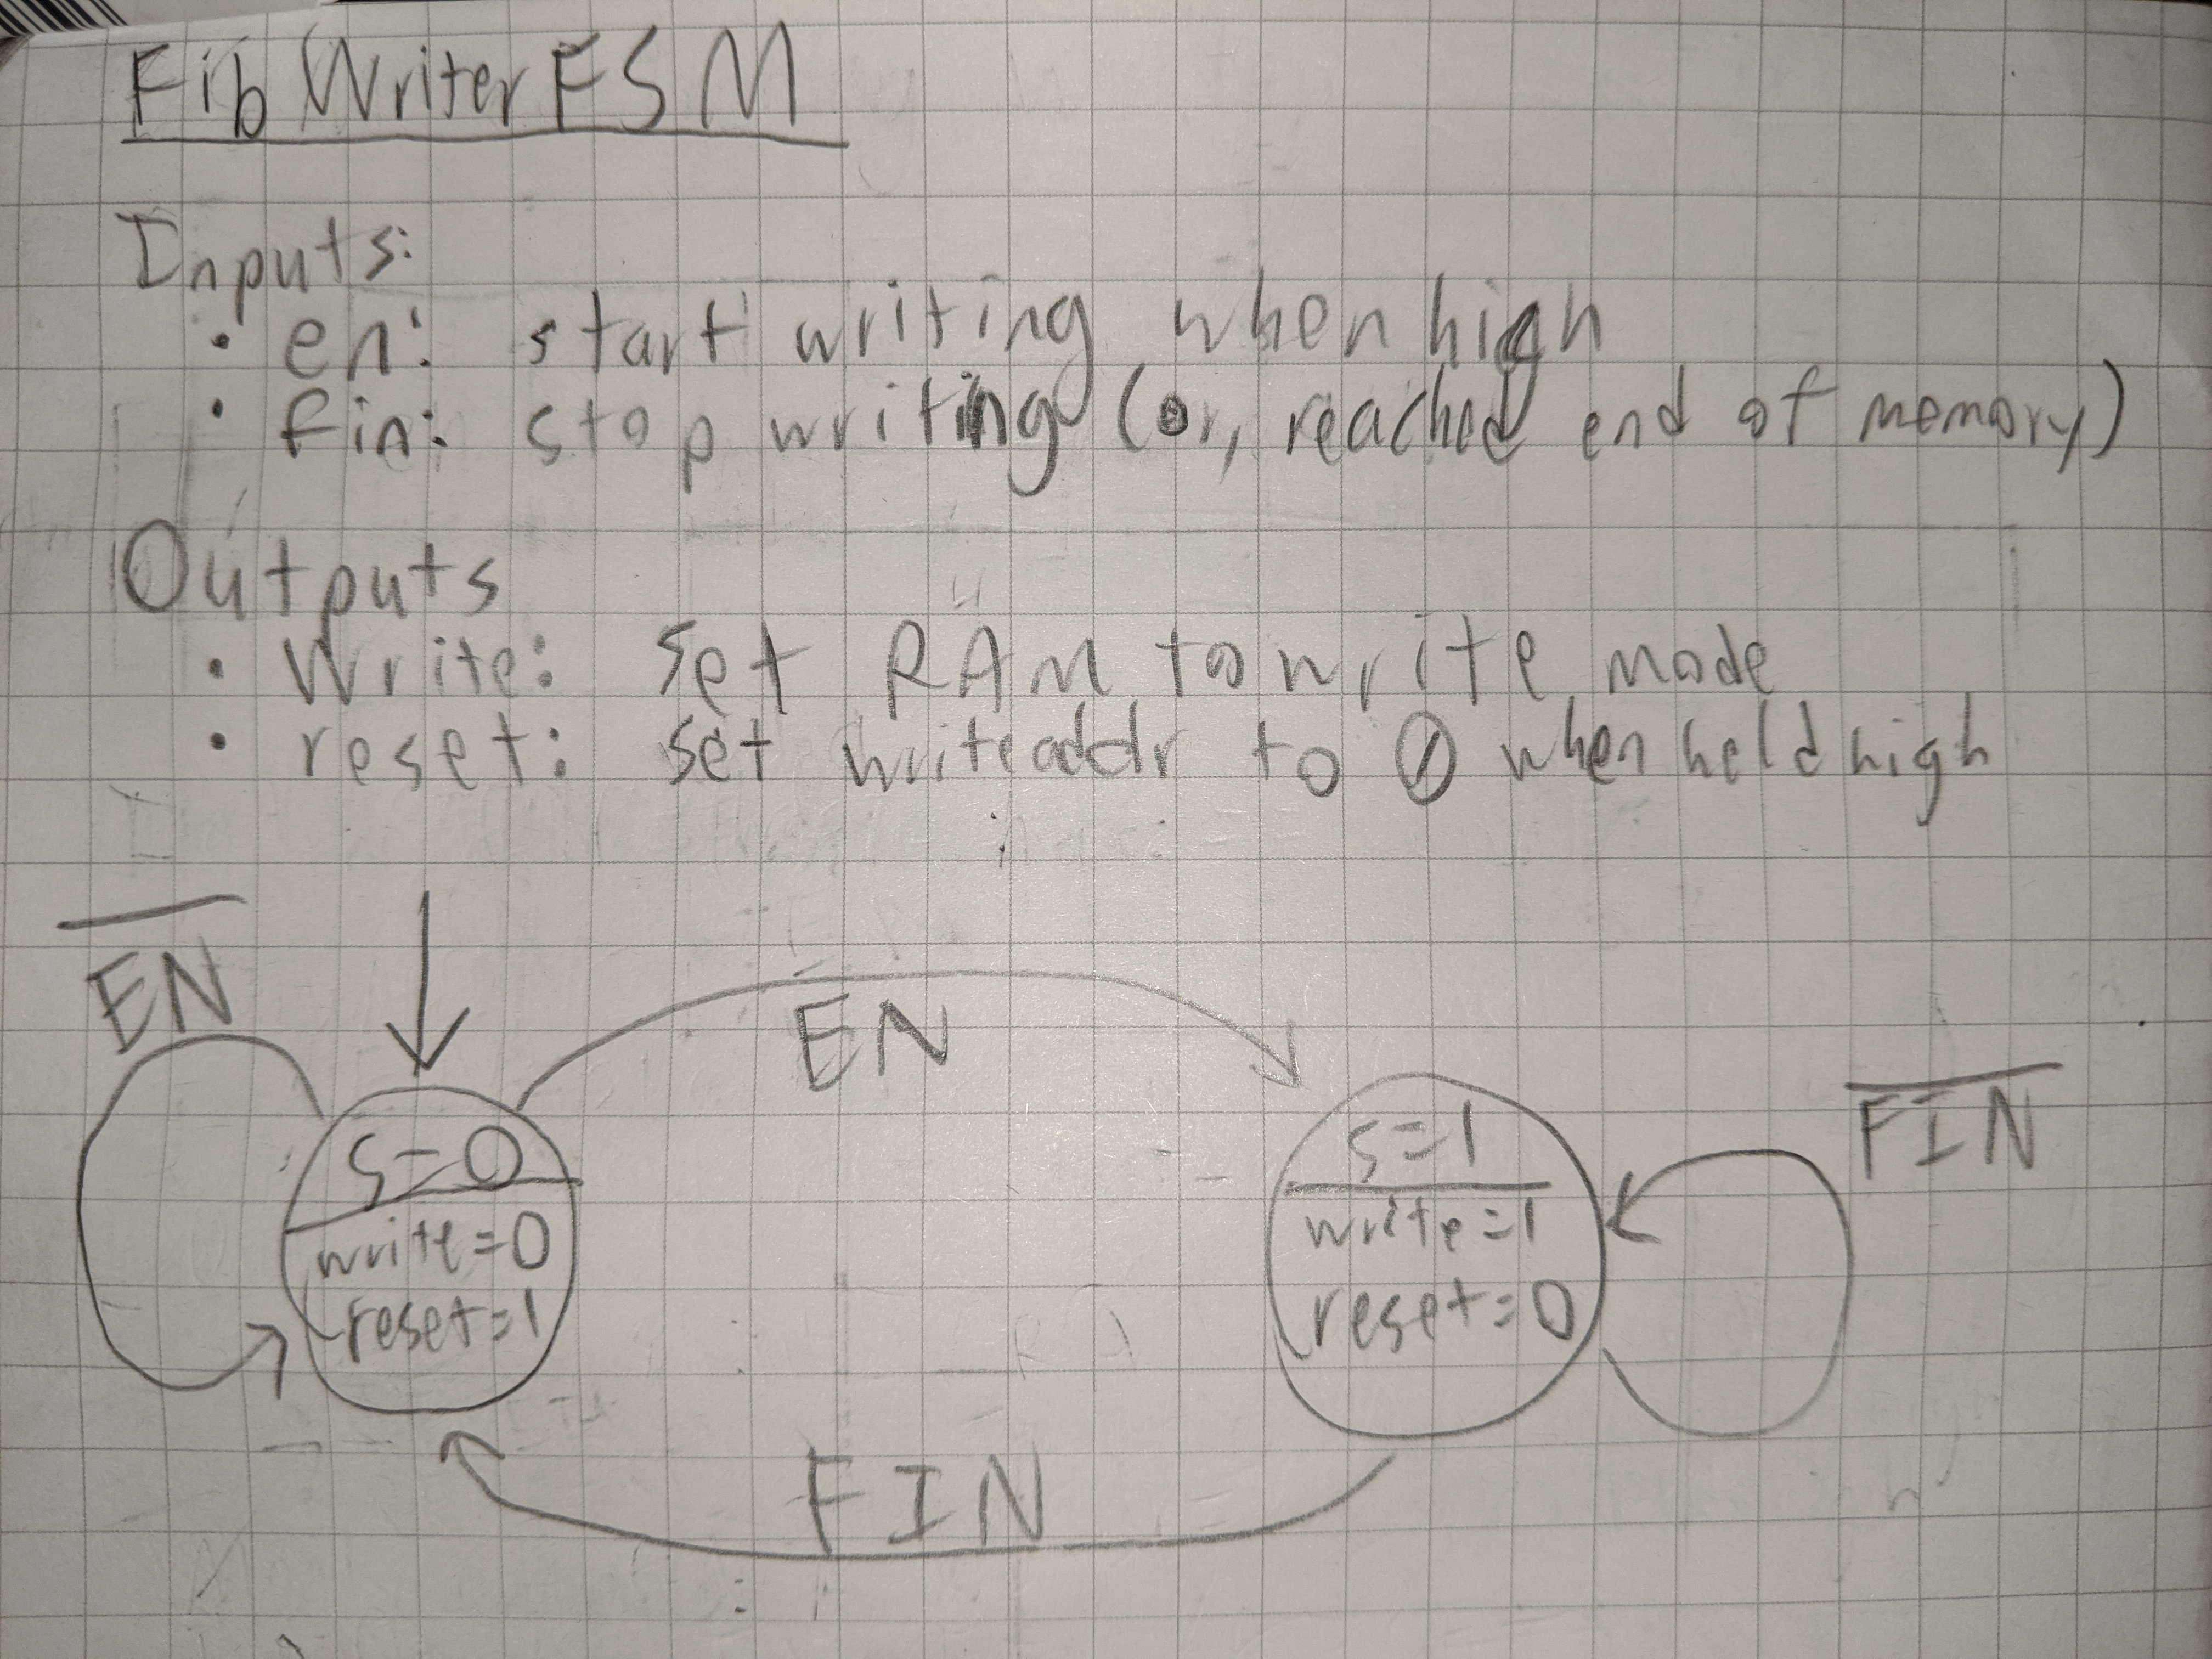
\includegraphics[width=\linewidth]{fsm-1.jpg}
\end{figure}

\section{Video}

See attached video file.

\end{document}